\chapter{Results: Sensitivity Analysis}
In this chapter, we use DYMOND and \Cyclus to conduct 
sensitivity analysis studies of the 
EG01-30 \gls{NFC} transition scenario. 
We use Dakota-\Cyclus (\texttt{dcwrapper}) 
and Dakota-DYMOND coupling (\texttt{ddwrapper}) toß
perform  
one-at-a-time sensitivity analysis (SA), synergistic 
SA, and global SA. 
This chapter has six sections: 
\begin{enumerate}
    \item Transition Scenario Specifications 
    \item Sensitivity Analysis Evaluation Metrics 
    \item One-at-a-time sensitivity analysis
    \item Synergistic sensitivity analysis
    \item Global sensitivity analysis
    \item Main Takeaways 
\end{enumerate}

\section{Transition Scenario Specification}
Both DYMOND and \Cyclus sensitivity analyses 
use the EG01-30 transition scenario.
Slight differences lie in the values of some input variables. 

\subsection{DYMOND}
The specifications of the EG01-30 transition scenario used in the 
DYMOND sensitivity analysis
are described in the DYMOND OECD benchmark transition 
scenario presented at the 17th Meeting of Expert Group on Advanced 
Fuel Cycle Scenarios in France in 2017 
\cite{oecd_nuclear_energy_agency_wpfc_nodate}. 
The OECD benchmark scenario is based on the EG01-30 transition scenario 
in which a \gls{PWR} fleet is transitioned to
a mixed fleet of \gls{MOX} \glspl{PWR} and \glspl{SFR}. 
Table \ref{tab:dymondinputs} describes high-level OECD benchmark transition 
scenario specifications. 

\begin{table}[]
    \centering
    \doublespacing
    \caption{OECD Benchmark Transition Scenario
	Specifications \cite{oecd_nuclear_energy_agency_wpfc_nodate}}
	\label{tab:dymondinputs}
    \small
    \begin{tabular}{ll}
    \hline
                               \textbf{Input Parameter}            & \textbf{Value}            \\ \hline
    Demand driving commodity   & Power              \\
                               Demand equation {[}TWhe/y{]}   & 430        \\
                               Transition Start Date [yr] & 80\\ 
                               Fleet share ratio [\%] & \gls{MOX} \gls{PWR}: 15\%, \gls{SFR}: 85\%\\ \hline
    \end{tabular}%
    \end{table}

\subsection{\Cyclus}
The \Cyclus transition scenario sensitivity analysis uses 
the linearly increasing power demand EG01-30 transition scenario 
(described in Section \ref{sec:eg01-30}).  
Figure \ref{fig:30flow} shows the facility and mass flow 
for this transition scenario in \Cyclus. 
Tables \ref{tab:bestinputs} and \ref{tab:facinputs}
shows the input parameters for \deploy and facilities
in the transition scenario. 
The \texttt{reactor} facility used in the \Cyclus simulation 
is a recipe reactor; it accepts a fresh fuel recipe and outputs 
a spent fuel recipe. 
The recipes used for the \gls{LWR}, \gls{MOX} \gls{LWR}, and 
\gls{SFR} are based on recipes generated by VISION 
\cite{chee_arfc/transition-scenarios_2018}
that closely match EG30 scenario specifications in 
Appendix B of the \gls{DOE} Evaluation and Screening Study 
(E\&S study) \cite{wigeland_nuclear_2014}. 

\begin{table}[]
    \centering
    \doublespacing
    \caption{\Cyclus facility input parameters for
	EG01-EG30 transition scenario
	that minimizes undersupply of power and minimizes 
	the undersupply and under capacity of other commodities. }
	\label{tab:facinputs}
    \small
    \begin{tabular}{llr}
        \hline
        \textbf{Facility}                 & \textbf{Input Parameter}                    & \textbf{Value} \\ \hline
        \multirow{4}{*}{\textbf{LWR}}     & Lifetime {[}months{]}              & 960   \\
                                 & Cycle time {[}months{]}            & 18    \\
                                 & Refuel time {[}months{]}           & 1     \\
                                 & Rated Power {[}MWe{]}              & 1000  \\ \hline
        \multirow{2}{*}{\textbf{MOX LWR}} & Lifetime {[}months{]}              & 960   \\
                                 & Cycle time {[}months{]}            & 18    \\
                                 & Refuel time {[}months{]}           & 1     \\
                                 & Rated Power {[}MWe{]}              & 1000  \\ \hline
        \multirow{4}{*}{\textbf{SFR}}     & Lifetime {[}months{]}              & 720   \\
                                 & Cycle time {[}months{]}            & 12    \\
                                 & Refuel time {[}months{]}           & 1     \\
                                 & Rated Power {[}MWe{]}              & 333   \\ \hline
        \textbf{Cooling Pools}            & Used fuel storage time {[}years{]} & 3  \\ \hline
        \end{tabular}
    \end{table}

\section{Sensitivity Analysis: Evaluation Metrics}
Evaluation metrics and their associated output variables 
must be defined to determine the basis of comparison for sensitivity 
analysis of \gls{NFC} transition scenarios.
The E\&S study \cite{wigeland_nuclear_2014} evaluated transition 
scenarios using nine metrics: nuclear waste 
management, proliferation risk, nuclear material security risk, 
safety, environmental impact, resource utilization, development 
and deployment risk, institutional issues, financial risk, and 
economics. 
These nine metrics are narrowed down into four categories: environmental 
impact, economics, proliferation risk and resource utilization
\cite{passerini_systematic_2014}. 

It is necessary to define output indicators to measure the 
impact of the variation of an input parameter on an output 
parameter \cite{noauthor_effects_2017}. 
Output indicators are introduced because of the need for a single value that 
is representative of the output parameter's time series.  
Four types of output indicators are introduced 
\cite{noauthor_effects_2017}: 
(1) the final value at the end of simulation
(2) the maximum value during simulation,  
(3) the cumulative sum over the whole simulation, and 
(4) the quality of Plutonium (equation \ref{eq:pu}). 
A different output indicator is used depending on 
the nature of the output parameter.

\begin{align}
    \label{eq:pu}
Quality\ of\ Pu = \frac{Pu_{239}+Pu_{241}}{Pu_{238}+Pu_{240}+Pu_{242}+Pu_{243}+Pu_{244}}
\end{align}

Table \ref{tab:category-output-DD} shows the four evaluation 
metrics and the associated output variables used in this work. 

\begin{table}[]
    \centering
    \doublespacing
    \caption {Evaluation metrics and their associated output 
    variables.}
	\label{tab:category-output-DD}
        \small
        \begin{tabular}{lll}	
            	\hline
            \textbf{Evaluation Metrics} & \textbf{Output Variable} & \textbf{Indicators}\\
            \hline
            \textbf{Waste Management} & \begin{tabular}[c]{@{}l@{}}High Level Waste Inventory\\ Depleted Uranium\end{tabular} & \begin{tabular}[c]{@{}l@{}}Final \\ Final \end{tabular}\\
            \hline
            \textbf{Proliferation Risk} &  \begin{tabular}[c]{@{}l@{}}Pu in Cooling Pools (CP)\\ Pu in HLW \\ Pu in Reprocessing Facilities (RPR) \\ 
            \end{tabular} & 
        \begin{tabular}[c]{@{}l@{}} Max, Quality\\ Max, Quality \\ Max, Quality \end{tabular} \\
            
            \hline
            \textbf{Resource Utilization} & Uranium Ore Used & Sum\\
            \hline
            \textbf{Goodness of Transition} & \begin{tabular}[c]{@{}l@{}}Total Idle Capacity\\ Date of Final Idle Capacity \\ Length of transition\end{tabular} & \begin{tabular}[c]{@{}l@{}}Sum \\ Final \\ -\end{tabular} \\ 
            \hline
            \end{tabular}
\end{table}

The operational conditions for the advanced reactors and
the specifics of the transition scenario are variable
since the fuel cycle simulator is modeling future 
trajectories. 
In the transition scenarios, we vary the following 
input parameters: 
\begin{itemize}
    \item Length of used fuel cooling time 
    \item Fleet share ratio of PWR MOX and SFR reactors 
	\item Introduction date of advanced reactor technology (Transition Year)
\end{itemize}

In the following sections, 
we conduct one-at-a-time, synergistic, and global
sensitivity analysis of these three input parameters and 
quantify the evaluation metric impact.  

\section{One-at-a-time Sensitivity Analysis}
\label{sec:oat}

\subsection{Length of cooling time for used fuel}
In the DYMOND and \Cyclus EG01-30 transition scenarios, 
we varied used fuel cooling time from 0 to 8 years. 
We compared these simulations based on the evaluation 
metrics described in Table \ref{tab:category-output-DD}.

\subsubsection{\textbf{DYMOND}}
Tables \ref{tab:dymond-ct-1} and \ref{tab:dymond-ct-2} show 
the absolute values of 
output variables associated with the environmental impact, 
resource utilization, and goodness of transition evaluation 
metrics for each scenario. 
Tables \ref{tab:dymond-ct-sa-1} and \ref{tab:dymond-ct-sa-2} 
show each scenario's percentage 
difference compared with the base case of `Cooling Time = 2 years'
scenario.

In Table \ref{tab:dymond-ct-1}, total idle capacity 
in the simulation increases for used fuel cooling time of 3 years 
onwards. 
This is because the fuel management strategy in the 
DYMOND OECD benchmark scenario was 
manually edited to work best with a 2 year used fuel cooling time.
The idle capacity in cooling time of 3 years onwards could be 
avoided by manually changing the fuel management strategy
in the DYMOND input file for the scenario. 
We did not manually change the fuel management strategy
because this is a one-at-a-time sensitivity analysis study 
and, thus, only used fuel cooling time was varied. 

In Table \ref{tab:dymond-ct-sa-2}, compared with the base case, 
as cooling time increases, maximum Pu in the cooling pools increases.
This is expected since there exists a larger inventory of used fuel 
in the cooling pools when cooling time increases. 
The quality of Pu in the cooling pools also increases as cooling time 
increases. 

\begin{table}[]
    \centering
    \onehalfspacing
    \caption{DYMOND: Assessment of how variation of used fuel cooling times
    impacts evaluation metrics (waste management, resource utilization, 
    and goodness of transition) for OECD benchmark transition scenario \cite{chee_gwenchee/ddwrapper_2019}.}
	\label{tab:dymond-ct-1}
        \footnotesize
        \begin{tabularx}{\textwidth}{R|RR|R|RRR}	
            \hline
            \textbf{Scenario} & \multicolumn{2}{c|}{\textbf{Environmental Impact}}                                                                                                                                                                                                                                                      & \textbf{Resource Utilization}                                                                                        & \multicolumn{3}{c}{\textbf{Goodness of Transition}}                                                                                                                                                                                 \\ \hline
\textbf{Used Fuel Cooling Time [yr]} & \textbf{Final HLW [kg] } & \textbf{Final Depleted U [kg]} &  \textbf{Uranium Ore Used [kg]}  & \textbf{Total Idle Capacity [kg]} & \textbf{Final Idle Capacity Year} & \textbf{Length of Transition [yrs]} \\ \hline
 0  &           1103.2 &                             916933.4 &                       16188.8 &                                    30148.8 &                      301 &                     227 \\ 
 1  &           1101.6 &                             916618.2 &                       16188.8 &                                    30148.8 &                      301 &                     227 \\ 
 2  &           1105.7 &                             916237.6 &                       16188.8 &                                    30148.8 &                      301 &                     227 \\ 
 3  &           1108.3 &                             916268.7 &                       16188.8 &                                   256588.8 &                      301 &                     227 \\ 
 4  &           1099.8 &                             916962.4 &                       16188.8 &                                 1338604.8 &                      301 &                     227 \\ \hline
\end{tabularx}%
\end{table}

\begin{table}[]
    \centering
    \onehalfspacing
    \caption{DYMOND: Assessment of how variation of used fuel cooling times
    impacts evaluation metrics (proliferation risk) for OECD benchmark
	transition scenario \cite{chee_gwenchee/ddwrapper_2019}.}
	\label{tab:dymond-ct-2}
    \footnotesize
        \begin{tabularx}{\textwidth}{R|RRRRRR}	
            \hline
            \textbf{Scenario} & \multicolumn{6}{c}{\textbf{Proliferation Risk}}  \\ \hline
\textbf{Used Fuel Cooling Time [yr]} & \textbf{Max Pu in CP [kg] } & \textbf{Quality at CP max Pu [kg]} &  \textbf{Max Pu in HLW [kg]}  & \textbf{Quality at HLW max Pu [kg]} & \textbf{Max Pu in RPR [kg]} & \textbf{Quality at RPR max Pu [kg]} \\ \hline
 0  &           0.0 &                             0 &                       18.374 &                                    0.650 &                      208.6 &                     - \\ 
 1  &           105.2 &                             0.652 &                       18.385 &                                    0.652 &                      208.6 &                     - \\ 
 2  &           196.8 &                             0.622 &                       18.409 &                                    0.653 &                      208.6 &                     - \\ 
 3  &           264.8 &                             0.659 &                       18.189 &                                   0.654 &                      208.6 &                     - \\ 
 4  &           348.2 &                             0.671 &                       16.805 &                                 0.658 &                      208.6 &                     - \\ \hline
\end{tabularx}%
\end{table}

\begin{table}[]
    \caption{DYMOND: Sensitivity analysis of how variation of used fuel 
    cooling times impacts evaluation metrics (waste management, resource utilization, 
    and goodness of transition) for OECD benchmark transition scenario.
    The numbers in the table represent the percentage difference between 
    an output variable from each scenario and the base case scenario (Cooling time = 2 years) \cite{chee_gwenchee/ddwrapper_2019}.}
    \label{tab:dymond-ct-sa-1}
    \onehalfspacing
    \footnotesize
    \begin{tabularx}{\textwidth}{R|RR|R|RRR}	
		\hline
        \textbf{Scenario} & \multicolumn{2}{c|}{\textbf{Environmental Impact}}                                    & \textbf{Resource Utilization}                                                                                       & \multicolumn{3}{c}{\textbf{Goodness of Transition}}                                                                                                                                                                                 \\ \hline
        \textbf{Used Fuel Cooling Time [yr]} & \textbf{Final HLW [\%] } & \textbf{Final Depleted U [\%]} &  \textbf{Uranium Ore Used [\%]]}  & \textbf{Total Idle Capacity [\%]} & \textbf{Final Idle Capacity Year [\%]} & \textbf{Length of Transition [\%]} \\ \hline
         0  &             \cellcolor[HTML]{67FD9A}-0.221736 &                                   \cellcolor[HTML]{67FD9A}0.075939 &                                                            \cellcolor[HTML]{67FD9A}0.0 &                 \cellcolor[HTML]{67FD9A}0.000000 &                                           \cellcolor[HTML]{67FD9A}0.0 & \cellcolor[HTML]{67FD9A}0.0 \\
		 1  &             \cellcolor[HTML]{67FD9A}-0.363540 &                                    \cellcolor[HTML]{67FD9A}0.041532 &                                                           \cellcolor[HTML]{67FD9A}0.0 &                 \cellcolor[HTML]{67FD9A}0.000000 &                                          \cellcolor[HTML]{67FD9A}0.0 & \cellcolor[HTML]{67FD9A}0.0 \\ 
		 2  &              \cellcolor[HTML]{000000}0.000000 &                                     \cellcolor[HTML]{000000}0.000000 &                                                              \cellcolor[HTML]{000000}0.0 &                 \cellcolor[HTML]{000000}0.000000 &                                         \cellcolor[HTML]{000000}0.0 & \cellcolor[HTML]{000000}0.0 \\ 
		 3  &              \cellcolor[HTML]{67FD9A}0.234524 &                                    \cellcolor[HTML]{67FD9A}0.003389 &                                                              \cellcolor[HTML]{67FD9A}0.0 &               \cellcolor[HTML]{FD6864}751.074670 &                                         \cellcolor[HTML]{67FD9A}0.0 & \cellcolor[HTML]{67FD9A}0.0 \\ 
		 4  &             \cellcolor[HTML]{67FD9A}-0.529033 &                                   \cellcolor[HTML]{67FD9A}0.079102 &                                                        \cellcolor[HTML]{67FD9A}0.0 &              \cellcolor[HTML]{FD6864}4339.993632 &                                        \cellcolor[HTML]{67FD9A}0.0 & \cellcolor[HTML]{67FD9A}0.0 \\ \hline
	\end{tabularx}%
    
    \resizebox{0.3\textwidth}{!}{
    \fbox{\begin{tabular}{ll}
        \textcolor{green}{$\blacksquare$} & $sensitivity \leq 1\%$ \\
        \textcolor{orange}{$\blacksquare$} & $1\% < sensitivity < 10\%$ \\
        \textcolor{red}{$\blacksquare$} & $sensitivity \geq 10\%$
        \end{tabular}}}
    \end{table}

    \begin{table}[]
        \caption{DYMOND: Sensitivity analysis of how variation of used fuel 
        cooling times impacts evaluation metrics (proliferation risk)for OECD benchmark transition scenario.
        The numbers in the table represent the percentage difference between 
    an output variable from each scenario and the base case scenario (Cooling time = 2 years) \cite{chee_gwenchee/ddwrapper_2019}.}
        \label{tab:dymond-ct-sa-2}
        \onehalfspacing
        \footnotesize
        \begin{tabularx}{\textwidth}{R|RRRRRR}	
            \hline
            \textbf{Scenario} & \multicolumn{6}{c}{\textbf{Proliferation Risk}}  \\ \hline
\textbf{Used Fuel Cooling Time [yr]} & \textbf{Max Pu in CP [\%] } & \textbf{Quality at CP max Pu [\%]} &  \textbf{Max Pu in HLW [\%]}  & \textbf{Quality at HLW max Pu [\%]} & \textbf{Max Pu in RPR [\%]} & \textbf{Quality at RPR max Pu [\%]} \\ \hline
             0  &             \cellcolor[HTML]{FD6864}-100 &                                   \cellcolor[HTML]{FD6864}-100 &                                                            \cellcolor[HTML]{67FD9A}-0.19 &                 \cellcolor[HTML]{67FD9A}-0.459 &                                           \cellcolor[HTML]{67FD9A}0.0 & \cellcolor[HTML]{67FD9A}- \\
             1  &             \cellcolor[HTML]{FD6864}-46.5 &                                    \cellcolor[HTML]{FE996B}4.82 &                                                           \cellcolor[HTML]{67FD9A}-0.13 &                 \cellcolor[HTML]{67FD9A}-0.153 &                                          \cellcolor[HTML]{67FD9A}0.0 & \cellcolor[HTML]{67FD9A}- \\ 
             2  &              \cellcolor[HTML]{000000}0.000000 &                                     \cellcolor[HTML]{000000}0.000000 &                                                              \cellcolor[HTML]{000000}0.0 &                 \cellcolor[HTML]{000000}0.000000 &                                         \cellcolor[HTML]{000000}0.0 & \cellcolor[HTML]{000000}0.0 \\ 
             3  &              \cellcolor[HTML]{FD6864}34.5 &                                    \cellcolor[HTML]{FE996B}5.95 &                                                              \cellcolor[HTML]{FE996B}-1.20 &               \cellcolor[HTML]{FD6864}0.153 &                                         \cellcolor[HTML]{67FD9A}0.0 & \cellcolor[HTML]{67FD9A}- \\ 
             4  &             \cellcolor[HTML]{FD6864}76.9 &                                   \cellcolor[HTML]{FE996B}7.88 &                                                        \cellcolor[HTML]{FE996B}-8.71 &              \cellcolor[HTML]{FD6864}0.766 &                                        \cellcolor[HTML]{67FD9A}0.0 & \cellcolor[HTML]{67FD9A}- \\ \hline
        \end{tabularx}%
        
        \resizebox{0.3\textwidth}{!}{
        \fbox{\begin{tabular}{ll}
            \textcolor{green}{$\blacksquare$} & $sensitivity \leq 1\%$ \\
            \textcolor{orange}{$\blacksquare$} & $1\% < sensitivity < 10\%$ \\
            \textcolor{red}{$\blacksquare$} & $sensitivity \geq 10\%$
            \end{tabular}}}
        \end{table}

    
\subsubsection{\textbf{\Cyclus}}

Tables \ref{tab:cyclus-ct-1} and \ref{tab:cyclus-ct-2} show 
the absolute values of 
output variables associated with the environmental impact, 
resource utilization, and goodness of transition evaluation 
metrics for each scenario. 
Tables \ref{tab:cyclus-ct-sa-1} and \ref{tab:cyclus-ct-sa-2} 
show each scenario's percentage 
difference compared with the base case of `Cooling Time = 2 years'
scenario.

In Table \ref{tab:cyclus-ct-sa-1}, most evaluation metrics do not change 
with variation in the used fuel cooling time, except for the final 
HLW amount. 
Final HLW amount decreases for a longer used fuel cooling time.
In Table \ref{tab:cyclus-ct-sa-2}, compared with the base case, 
as cooling time increases, maximum Pu in the cooling pools increases.
This is similar to the result for the DYMOND transition scenario (table 
\ref{tab:dymond-ct-sa-2}). 
This is expected since there will be a larger inventory of used fuel 
in the cooling pools when cooling time increases. 
The quality of Pu in the cooling pools decreases as cooling time 
increases. 
Maximum Pu in HLW and reprocessing facilities, and their corresponding 
Pu quality, decrease for a longer cooling time. 

\begin{table}[]
    \centering
    \onehalfspacing
    \caption{\Cyclus: Assessment of how variation of used fuel cooling times
    impacts evaluation metrics (waste management, resource utilization, 
    and goodness of transition) for OECD benchmark transition scenario \cite{chee_arfc/dcwrapper_2019}.}
	\label{tab:cyclus-ct-1}
        \footnotesize
        \begin{tabularx}{\textwidth}{R|RR|R|RRR}
            \hline	
            \textbf{Scenario} & \multicolumn{2}{c|}{\textbf{Environmental Impact}}                                                                                                                                                                                                                                                      & \textbf{Resource Utilization}                                                                                        & \multicolumn{3}{c}{\textbf{Goodness of Transition}}                                                                                                                                                                                 \\ \hline
\textbf{Used Fuel Cooling Time [yr]} & \textbf{Final HLW [kg] } & \textbf{Final Depleted U [kg]} &  \textbf{Uranium Ore Used [kg]}  & \textbf{Total Idle Capacity [kg]} & \textbf{Final Idle Capacity Year} & \textbf{Length of Transition [yrs]} \\ \hline

0  & 13223828.1 & 798818620.4      & 1.437e11    & 135.1               & 962                     & 2                      \\
2  & 13073261.2 & 798818620.4      & 1.437e11    & 135.1               & 962                     & 2                      \\
4  & 12906058.3 & 798818620.4      & 1.437e11    & 135.1               & 962                     & 2                      \\
6  & 12795682.5 & 798818620.4      & 1.437e11    & 135.1               & 962                     & 2                      \\
8  & 12726528.6 & 798818620.4      & 1.437e11    & 135.1               & 962                     & 2                     \\ \hline 
        \end{tabularx}
\end{table}

\begin{table}[]
    \centering
    \onehalfspacing
    \caption{\Cyclus: Assessment of how variation of used fuel cooling times
    impacts evaluation metrics (proliferation risk) for OECD benchmark
	transition scenario \cite{chee_arfc/dcwrapper_2019}.}
	\label{tab:cyclus-ct-2}
    \footnotesize
        \begin{tabularx}{\textwidth}{R|RRRRRR}	
            \hline
            \textbf{Scenario} & \multicolumn{6}{c}{\textbf{Proliferation Risk}}  \\ \hline
\textbf{Used Fuel Cooling Time [yr]} & \textbf{Max Pu in CP [kg] } & \textbf{Quality at CP max Pu [kg]} &  \textbf{Max Pu in HLW [kg]}  & \textbf{Quality at HLW max Pu [kg]} & \textbf{Max Pu in RPR [kg]} & \textbf{Quality at RPR max Pu [kg]} \\ \hline
0  & 48979.28         & 0.66                           & 44426.65      & 0.62                        & 2800580.69        & 0.49                            \\
2  & 199036.06        & 0.6                            & 43629.18      & 0.62                        & 2637125.07        & 0.48                            \\
4  & 368405.04        & 0.58                           & 42844.4       & 0.62                        & 2460403.99        & 0.48                            \\
6  & 554321.66        & 0.57                           & 42646.72      & 0.62                        & 2290857.92        & 0.47                            \\
8  & 733483.85        & 0.56                           & 42858.1       & 0.62                        & 2111786.28        & 0.47                           \\ \hline
\end{tabularx}%
\end{table}

% add color 
\begin{table}[]
    \onehalfspacing
    \caption{\Cyclus: Sensitivity analysis of how variation of used fuel 
    cooling times impacts evaluation metrics (environmental impact, resource
    utilization, and goodness of transition) for OECD benchmark 
    transition scenario.
    The numbers in the table represent the percentage difference between 
    an output variable from each scenario and the base case scenario (Cooling time = 2 years) \cite{chee_arfc/dcwrapper_2019}.}
    \label{tab:cyclus-ct-sa-1}
    \footnotesize
    \begin{tabularx}{\textwidth}{R|RR|R|RRR}	
		\hline
        \textbf{Scenario} & \multicolumn{2}{c|}{\textbf{Environmental Impact}}                                    & \textbf{Resource Utilization}                                                                                       & \multicolumn{3}{c}{\textbf{Goodness of Transition}}                                                                                                                                                                                 \\ \hline
        \textbf{Used Fuel Cooling Time [yr]} & \textbf{Final HLW [\%] } & \textbf{Final Depleted U [\%]} &  \textbf{Uranium Ore Used [\%]]}  & \textbf{Total Idle Capacity [\%]} & \textbf{Final Idle Capacity Year [\%]} & \textbf{Length of Transition [\%]} \\ \hline0  & \cellcolor[HTML]{FE996B}1.15      & \cellcolor[HTML]{67FD9A}0.0              & \cellcolor[HTML]{67FD9A}0.0               & \cellcolor[HTML]{67FD9A}0.0                 & \cellcolor[HTML]{67FD9A}0.0                     & \cellcolor[HTML]{67FD9A}0.0                    \\
        2  & \cellcolor[HTML]{000000}0.0       & \cellcolor[HTML]{000000}0.0              & \cellcolor[HTML]{000000}0.0               & \cellcolor[HTML]{000000}0.0                 & \cellcolor[HTML]{000000}0.0                     & \cellcolor[HTML]{000000}0.0                    \\
        4  & \cellcolor[HTML]{FE996B}-1.28       & \cellcolor[HTML]{67FD9A}0.0              & \cellcolor[HTML]{67FD9A}0.0               & \cellcolor[HTML]{67FD9A}0.0                 & \cellcolor[HTML]{67FD9A}0.0                     & \cellcolor[HTML]{67FD9A}0.0                    \\
        6  & \cellcolor[HTML]{FE996B}-2.12     & \cellcolor[HTML]{67FD9A}0.0              & \cellcolor[HTML]{67FD9A}0.0               & \cellcolor[HTML]{67FD9A}0.0                 & \cellcolor[HTML]{67FD9A}0.0                     & \cellcolor[HTML]{67FD9A}0.0                    \\
        8  & \cellcolor[HTML]{FE996B}-2.65     & \cellcolor[HTML]{67FD9A}0.0              & \cellcolor[HTML]{67FD9A}0.0               & \cellcolor[HTML]{67FD9A}0.0                 & \cellcolor[HTML]{67FD9A}0.0                     & \cellcolor[HTML]{67FD9A}0.0                   \\ \hline 
                \end{tabularx}%
    
    \resizebox{0.3\textwidth}{!}{
    \fbox{\begin{tabular}{ll}
        \textcolor{green}{$\blacksquare$} & $sensitivity \leq 1\%$ \\
        \textcolor{orange}{$\blacksquare$} & $1\% < sensitivity < 10\%$ \\
        \textcolor{red}{$\blacksquare$} & $sensitivity \geq 10\%$
        \end{tabular}}}
    \end{table}

    \begin{table}[]
        \onehalfspacing
        \caption{\Cyclus: Sensitivity analysis of how variation of used fuel 
        cooling times impacts evaluation metrics (proliferation risk) for OECD benchmark transition scenario.
        The numbers in the table represent the percentage difference between 
        an output variable from each scenario and the base case scenario (Cooling time = 2 years) \cite{chee_arfc/dcwrapper_2019}.}
        \label{tab:cyclus-ct-sa-2}
        \footnotesize
        \begin{tabularx}{\textwidth}{R|RRRRRR}	
            \hline
            \textbf{Scenario} & \multicolumn{6}{c}{\textbf{Proliferation Risk}}  \\ \hline
            \textbf{Used Fuel Cooling Time [yr]} & \textbf{Max Pu in CP [\%] } & \textbf{Quality at CP max Pu [\%]} &  \textbf{Max Pu in HLW [\%]}  & \textbf{Quality at HLW max Pu [\%]} & \textbf{Max Pu in RPR [\%]} & \textbf{Quality at RPR max Pu [\%]} \\ \hline
            0  & \cellcolor[HTML]{FD6864}-75.39           & \cellcolor[HTML]{FE996B}8.99                           & \cellcolor[HTML]{FE996B}1.83          & \cellcolor[HTML]{67FD9A}0.08                        & \cellcolor[HTML]{FE996B}6.2               & \cellcolor[HTML]{FE996B}1.45                            \\
2  &\cellcolor[HTML]{000000}0.0              & \cellcolor[HTML]{000000}0.0                            & \cellcolor[HTML]{000000}0.0           & \cellcolor[HTML]{000000}0.0                         & \cellcolor[HTML]{000000}0.0               & \cellcolor[HTML]{000000}0.0                             \\
4  & \cellcolor[HTML]{FD6864}85.09            & \cellcolor[HTML]{FE996B}-3.34                          & \cellcolor[HTML]{FE996B}-1.8          & \cellcolor[HTML]{67FD9A}-0.12                       & \cellcolor[HTML]{FE996B}-6.7              & \cellcolor[HTML]{FE996B}-1.06                           \\
6  & \cellcolor[HTML]{FD6864}178.5            & \cellcolor[HTML]{FE996B}-5.55                          & \cellcolor[HTML]{FE996B}-2.25         & \cellcolor[HTML]{67FD9A}-0.15                       & \cellcolor[HTML]{FD6864}-13.13            & \cellcolor[HTML]{FE996B}-2.11                           \\
8  & \cellcolor[HTML]{FD6864}268.52           & \cellcolor[HTML]{FE996B}-7.23                          & \cellcolor[HTML]{FE996B}-1.77         & \cellcolor[HTML]{67FD9A}-0.22                       & \cellcolor[HTML]{FD6864}-19.92            & \cellcolor[HTML]{FE996B}-3.0                           \\ \hline
        \end{tabularx}
        \resizebox{0.3\textwidth}{!}{
            \fbox{\begin{tabular}{ll}
                \textcolor{green}{$\blacksquare$} & $sensitivity \leq 1\%$ \\
                \textcolor{orange}{$\blacksquare$} & $1\% < sensitivity < 10\%$ \\
                \textcolor{red}{$\blacksquare$} & $sensitivity \geq 10\%$
                \end{tabular}}}
        \end{table}

\subsection{Fleet share ratio of PWR MOX and SFR reactors}

The fleet share ratio of \gls{MOX} \glspl{PWR} and \glspl{SFR}
was varied from 0\% to 20\% of \gls{MOX} \glspl{PWR} for the 
\Cyclus EG01-30 transition scenario. 
We compared these simulations based on the evaluation 
metrics described in Table \ref{tab:category-output-DD}. 

Tables \ref{tab:cyclus-fs-1} and \ref{tab:cyclus-fs-2} show 
the absolute values of 
output variables associated with the environmental impact, 
resource utilization, and goodness of transition evaluation 
metrics for each scenario. 
Tables \ref{tab:cyclus-fs-sa-1} and \ref{tab:cyclus-fs-sa-2} 
show each scenario's percentage 
difference compared with the base case of `Fleet share = 15\% 
\gls{MOX} \glspl{PWR}' scenario. 

In Table \ref{tab:cyclus-fs-sa-1}, most evaluation metrics do not change 
for variation in fleet share ratio, except for the final 
amount of HLW in the scenario. 
The final amount of HLW is largest for 0\% fleet share of \gls{MOX} 
\glspl{PWR} and decreases as the fleet share of \gls{MOX} \glspl{PWR} 
increases. 
In Table \ref{tab:cyclus-fs-sa-2}, maximum Pu in cooling pools and 
reprocessing facility 
decreases for increasing fleet share ratio of \gls{MOX} \glspl{PWR}; 
however, the quality of Pu increases. 
Maximum Pu in HLW increases for a decreasing fleet share ratio
of \gls{MOX} \glspl{PWR}, while the quality of Pu decreases slightly.
Therefore, if minimizing proliferation risk is a high priority, 
a transition scenario 
with a smaller fleet share of \gls{MOX} \glspl{PWR} is recommended
to minimize the Pu amount in the cooling pools and reprocessing facilities. 

% correct stuff 
\begin{table}[]
    \centering
    \onehalfspacing
    \caption{\Cyclus: Assessment of how variation of fleet share ratio
    of PWR MOX and SFR reactors
    impacts evaluation metrics (environmental impact, resource
    utilization, and goodness of transition) for EG01-30 transition scenario \cite{chee_arfc/dcwrapper_2019}.}
	\label{tab:cyclus-fs-1}
    \footnotesize
        \begin{tabularx}{\textwidth}{R|RR|R|RRR}
            \hline	
            \textbf{Scenario} & \multicolumn{2}{c|}{\textbf{Environmental Impact}}                                                                                                                                                                                                                                                      & \textbf{Resource Utilization}                                                                                        & \multicolumn{3}{c}{\textbf{Goodness of Transition}}                                                                                                                                                                                 \\ \hline
\textbf{MOX Fleet Share [\%]} & \textbf{Final HLW [kg] } & \textbf{Final Depleted U [kg]} &  \textbf{Uranium Ore Used [kg]}  & \textbf{Total Idle Capacity [kg]} & \textbf{Final Idle Capacity Year} & \textbf{Length of Transition [yrs]} \\ \hline

0  & 13153061.6 & 798818620.4      & 1.437e11    & 135.1               & 962                     & 2                      \\
5  & 13056988.7 & 798818620.4      & 1.437e11    & 135.1               & 962                     & 2                      \\
10 & 13051896.3 & 798818620.4      & 1.437e11    & 135.1               & 962                     & 2                      \\
15 & 12959554.1 & 798818620.4      & 1.437e11    & 135.1               & 962                     & 2                      \\
20 & 13002120.9 & 798818620.4      & 1.437e11    & 135.1               & 962                     & 2                     \\ \hline
        \end{tabularx}
\end{table}

% correct stuff 
\begin{table}[]
    \onehalfspacing
    \centering
    \caption{\Cyclus: Assessment of how variation of fleet share ratio
    of PWR MOX and SFR reactors
    impacts evaluation metrics (proliferation risk) for EG01-30 transition scenario \cite{chee_arfc/dcwrapper_2019}.}
	\label{tab:cyclus-fs-2}
    \footnotesize
        \begin{tabularx}{\textwidth}{R|RRRRRR}	
            \hline
            \textbf{Scenario} & \multicolumn{6}{c}{\textbf{Proliferation Risk}}  \\ \hline
\textbf{MOX Fleet Share [\%]} & \textbf{Max Pu in CP [kg] } & \textbf{Quality at CP max Pu [kg]} &  \textbf{Max Pu in HLW [kg]}  & \textbf{Quality at HLW max Pu [kg]} & \textbf{Max Pu in RPR [kg]} & \textbf{Quality at RPR max Pu [kg]} \\ \hline
0  & 256794.03        & 0.66                           & 45816.02      & 0.62                        & 2357604.01        & 0.55                            \\
5  & 273733.13        & 0.62                           & 44338.72      & 0.62                        & 2461421.31        & 0.51                            \\
10 & 279694.78        & 0.61                           & 44055.54      & 0.62                        & 2513133.76        & 0.5                             \\
15 & 285794.85        & 0.59                           & 42905.59      & 0.62                        & 2552142.82        & 0.48                            \\
20 & 291786.54        & 0.58                           & 43133.61      & 0.62                        & 2605589.02        & 0.47                           \\ \hline
\end{tabularx}%
\end{table}

% correct stuff 
\begin{table}[]
    \onehalfspacing
    \caption{\Cyclus: Sensitivity analysis of how variation of fleet share 
    ratio impacts evaluation metrics (environmental impact, resource
    utilization, and goodness of transition) for OECD benchmark 
    transition scenario.
    The numbers in the table represent the percentage difference between 
    an output variable from each scenario and the base case scenario 
    (PWR MOX fleet share = 15\%) \cite{chee_arfc/dcwrapper_2019}.}
    \label{tab:cyclus-fs-sa-1}
    \footnotesize
    \begin{tabularx}{\textwidth}{R|RR|R|RRR}	
		\hline
        \textbf{Scenario} & \multicolumn{2}{c|}{\textbf{Environmental Impact}}                                    & \textbf{Resource Utilization}                                                                                       & \multicolumn{3}{c}{\textbf{Goodness of Transition}}                                                                                                                                                                                 \\ \hline
        \textbf{MOX Fleet Share [\%]} & \textbf{Final HLW [\%] } & \textbf{Final Depleted U [\%]} &  \textbf{Uranium Ore Used [\%]]}  & \textbf{Total Idle Capacity [\%]} & \textbf{Final Idle Capacity Year [\%]} & \textbf{Length of Transition [\%]} \\ \hline
        0  & \cellcolor[HTML]{FE996B}1.49      & \cellcolor[HTML]{67FD9A}0.0              & \cellcolor[HTML]{67FD9A}0.0               & \cellcolor[HTML]{67FD9A}0.0                 & \cellcolor[HTML]{67FD9A}0.0                     & \cellcolor[HTML]{67FD9A}0.0                    \\
        5  & \cellcolor[HTML]{67FD9A}0.75      & \cellcolor[HTML]{67FD9A}0.0              & \cellcolor[HTML]{67FD9A}0.0               & \cellcolor[HTML]{67FD9A}0.0                 & \cellcolor[HTML]{67FD9A}0.0                     & \cellcolor[HTML]{67FD9A}0.0                    \\
        10 & \cellcolor[HTML]{67FD9A}0.71      & \cellcolor[HTML]{67FD9A}0.0              & \cellcolor[HTML]{67FD9A}0.0               & \cellcolor[HTML]{67FD9A}0.0                 & \cellcolor[HTML]{67FD9A}0.0                     & \cellcolor[HTML]{67FD9A}0.0                    \\
        15 & \cellcolor[HTML]{000000}0.0       & \cellcolor[HTML]{000000}0.0              & \cellcolor[HTML]{000000}0.0               & \cellcolor[HTML]{000000}0.0                 & \cellcolor[HTML]{000000}0.0                     & \cellcolor[HTML]{000000}0.0                    \\
        20 & \cellcolor[HTML]{67FD9A}0.33      & \cellcolor[HTML]{67FD9A}0.0              & \cellcolor[HTML]{67FD9A}0.0               & \cellcolor[HTML]{67FD9A}0.0                 & \cellcolor[HTML]{67FD9A}0.0                     & \cellcolor[HTML]{67FD9A}0.0                   \\ \hline
                       \end{tabularx}%
    
    \resizebox{0.3\textwidth}{!}{
    \fbox{\begin{tabular}{ll}
        \textcolor{green}{$\blacksquare$} & $sensitivity \leq 1\%$ \\
        \textcolor{orange}{$\blacksquare$} & $1\% < sensitivity < 10\%$ \\
        \textcolor{red}{$\blacksquare$} & $sensitivity \geq 10\%$
        \end{tabular}}}
    \end{table}

    % correct stuff 
\begin{table}[]
    \onehalfspacing
    \caption{\Cyclus: Sensitivity analysis of how variation of fleet share 
    ratio impacts evaluation metrics (proliferation risk) for OECD benchmark 
    transition scenario.
    The numbers in the table represent the percentage difference between 
    an output variable from each scenario and the base case scenario
    (PWR MOX fleet share = 15\%) \cite{chee_arfc/dcwrapper_2019}.}
    \label{tab:cyclus-fs-sa-2}
    \footnotesize
    \begin{tabularx}{\textwidth}{R|RRRRRR}	
		\hline
        \textbf{Scenario} & \multicolumn{6}{c}{\textbf{Proliferation Risk}}  \\ \hline
        \textbf{MOX Fleet Share [\%]} & \textbf{Max Pu in CP [\%] } & \textbf{Quality at CP max Pu [\%]} &  \textbf{Max Pu in HLW [\%]}  & \textbf{Quality at HLW max Pu [\%]} & \textbf{Max Pu in RPR [\%]} & \textbf{Quality at RPR max Pu [\%]} \\ \hline
0  & \cellcolor[HTML]{FD6864}-10.15           & \cellcolor[HTML]{FD6864}10.63                          & \cellcolor[HTML]{FE996B}6.78          & \cellcolor[HTML]{67FD9A}-0.48                       & \cellcolor[HTML]{FE996B}-7.62             & \cellcolor[HTML]{FD6864}14.05                           \\
        5  & \cellcolor[HTML]{FE996B}-4.22            & \cellcolor[HTML]{FE996B}4.34                           & \cellcolor[HTML]{FE996B}3.34          & \cellcolor[HTML]{67FD9A}-0.21                       & \cellcolor[HTML]{FE996B}-3.55             & \cellcolor[HTML]{FE996B}6.57                            \\
        10 & \cellcolor[HTML]{FE996B}-2.13            & \cellcolor[HTML]{FE996B}2.15                           & \cellcolor[HTML]{FE996B}2.68          & \cellcolor[HTML]{67FD9A}-0.09                       & \cellcolor[HTML]{FE996B}-1.53             & \cellcolor[HTML]{FE996B}3.35                            \\
        15 & \cellcolor[HTML]{000000}0.0              & \cellcolor[HTML]{000000}0.0                            & \cellcolor[HTML]{000000}0.0           & \cellcolor[HTML]{000000}0.0                         & \cellcolor[HTML]{000000}0.0               & \cellcolor[HTML]{000000}0.0                             \\
        20 & \cellcolor[HTML]{FE996B}2.1              & \cellcolor[HTML]{FE996B}-2.02                          & \cellcolor[HTML]{67FD9A}0.53          & \cellcolor[HTML]{67FD9A}0.13                        & \cellcolor[HTML]{FE996B}2.09              & \cellcolor[HTML]{FE996B}-2.9                           \\ \hline
                           \end{tabularx}%
    
    \resizebox{0.3\textwidth}{!}{
    \fbox{\begin{tabular}{ll}
        \textcolor{green}{$\blacksquare$} & $sensitivity \leq 1\%$ \\
        \textcolor{orange}{$\blacksquare$} & $1\% < sensitivity < 10\%$ \\
        \textcolor{red}{$\blacksquare$} & $sensitivity \geq 10\%$
        \end{tabular}}}
    \end{table}


\subsection{Introduction year of advanced reactor technology}
The introduction year of advanced reactor technology
was varied from year 80 to 84 for the \Cyclus 
EG01-30 transition scenario. 
We compared these simulations based on the evaluation 
metrics described in Table \ref{tab:category-output-DD}.

Tables \ref{tab:cyclus-ty-1} and \ref{tab:cyclus-ty-2} show 
the absolute values of 
output variables associated with the environmental impact, 
resource utilization, and goodness of transition evaluation 
metrics for each scenario. 
Tables \ref{tab:cyclus-ty-sa-1} and \ref{tab:cyclus-ty-sa-2} 
show each scenario's percentage 
difference compared with the base case of `Transition Year = 80'
scenario. 

In Table \ref{tab:cyclus-ty-sa-1}, total idle capacity 
in the simulation is minimized at an advanced reactor 
introduction year of 82 onwards. 
Final HLW and depleted uranium increases for a later 
advanced reactor introduction year.
In Table \ref{tab:cyclus-ty-sa-2}, maximum Pu in cooling 
pools has a mostly constant trend after advanced reactor 
introduction year of 80. 
For a later advanced reactor introduction year, 
maximum Pu in HLW increases, while maximum Pu in reprocessing facilities 
decreases; the quality of Pu is constant. 
A later advanced reactor introduction year should be 
selected to ensure minimal idle capacity.

% correct stuff
\begin{table}[]
    \centering
    \onehalfspacing
    \caption{\Cyclus: Assessment of how variation of introduction date of 
    advanced reactor technology
    impacts evaluation metrics (environmental impact, resource
    utilization, and goodness of transition) for EG01-30 transition scenario \cite{chee_arfc/dcwrapper_2019}.}
	\label{tab:cyclus-ty-1}
        \footnotesize
        \begin{tabularx}{\textwidth}{R|RR|R|RRR}
            \hline	
            \textbf{Scenario} & \multicolumn{2}{c|}{\textbf{Environmental Impact}}                                                                                                                                                                                                                                                      & \textbf{Resource Utilization}                                                                                        & \multicolumn{3}{c}{\textbf{Goodness of Transition}}                                                                                                                                                                                 \\ \hline
\textbf{Transition Year} & \textbf{Final HLW [kg] } & \textbf{Final Depleted U [kg]} &  \textbf{Uranium Ore Used [kg]}  & \textbf{Total Idle Capacity [MW]} & \textbf{Final Idle Capacity Year} & \textbf{Length of Transition [yrs]} \\ \hline

80  & 12959554.6 & 798818620.4      & 1.437e11    & 135.1               & 962                     & 2                      \\
81  & 13069177.0 & 798818620.4      & 1.437e11    & 120.9               & 972                     & 0                      \\
82  & 13220184.0 & 803332630.7      & 1.437e11    & 121.1               & 980                     & 0                      \\
83  & 13360033.7 & 807846641.1      & 1.437e11    & 121.1               & 980                     & 0                      \\
84 & 13337086.8 & 807846641.1      & 1.437e11    & 121.1               & 980                     & 0                     \\ \hline
        \end{tabularx}
\end{table}

% correct stuff 
\begin{table}[]
    \centering
    \onehalfspacing
    \caption{\Cyclus: Assessment of how variation of introduction date of 
    advanced reactor technology
    impacts evaluation metrics (proliferation risk) 
    for EG01-30 transition scenario \cite{chee_arfc/dcwrapper_2019}.}
	\label{tab:cyclus-ty-2}
    \footnotesize
        \begin{tabularx}{\textwidth}{R|RRRRRR}
            \hline	
            \textbf{Scenario} & \multicolumn{6}{c}{\textbf{Proliferation Risk}}  \\ \hline
            \textbf{Transition Year} & \textbf{Max Pu in CP [kg] } & \textbf{Quality at CP max Pu [kg]} &  \textbf{Max Pu in HLW [kg]}  & \textbf{Quality at HLW max Pu [kg]} & \textbf{Max Pu in RPR [kg]} & \textbf{Quality at RPR max Pu [kg]} \\ \hline
            80  & 285794.85        & 0.59                           & 42905.59      & 0.62                        & 2552142.82        & 0.48                            \\
81  & 269666.8         & 0.60                            & 44291.11      & 0.62                        & 2530146.38        & 0.48                            \\
82  & 273313.41        & 0.60                            & 45673.72      & 0.62                        & 2489776.12        & 0.48                            \\
83  & 273307.72        & 0.59                           & 46848.37      & 0.62                        & 2475855.63        & 0.48                            \\
84 & 269414.41        & 0.60                            & 46714.21      & 0.62                        & 2455878.54        & 0.48                           \\ \hline
        \end{tabularx}
\end{table}

% correct stuff
\begin{table}[]
    \onehalfspacing
    \caption{\Cyclus: Sensitivity analysis of how variation of advanced reactor 
    introduction year impacts evaluation metrics (environmental impact, resource
    utilization, and goodness of transition) for OECD benchmark 
    transition scenario.
    The numbers in the table represent the percentage difference between 
    an output variable from each scenario and the base case scenario
    (transition year = 80) \cite{chee_arfc/dcwrapper_2019}.}
    \label{tab:cyclus-ty-sa-1}
    \footnotesize
    \begin{tabularx}{\textwidth}{R|RR|R|RRR}	
		\hline
        \textbf{Scenario} & \multicolumn{2}{c|}{\textbf{Environmental Impact}}                                    & \textbf{Resource Utilization}                                                                                       & \multicolumn{3}{c}{\textbf{Goodness of Transition}}                                                                                                                                                                                 \\ \hline
        \textbf{Transition Year} & \textbf{Final HLW [\%] } & \textbf{Final Depleted U [\%]} &  \textbf{Uranium Ore Used [\%]]}  & \textbf{Total Idle Capacity [\%]} & \textbf{Final Idle Capacity Year [\%]} & \textbf{Length of Transition [\%]} \\ \hline
        80  & \cellcolor[HTML]{000000}0.0       & \cellcolor[HTML]{000000}0.0              & \cellcolor[HTML]{000000}0.0               & \cellcolor[HTML]{000000}0.0                 & \cellcolor[HTML]{000000}0.0                     & \cellcolor[HTML]{000000}0.0                    \\
        81  & \cellcolor[HTML]{67FD9A}0.85      & \cellcolor[HTML]{67FD9A}0.0              & \cellcolor[HTML]{67FD9A}0.0               & \cellcolor[HTML]{FD6864}-10.51              & \cellcolor[HTML]{FE996B}1.04                    & \cellcolor[HTML]{FD6864}-100.0                 \\
        82  & \cellcolor[HTML]{FE996B}2.01      & \cellcolor[HTML]{67FD9A}0.57             & \cellcolor[HTML]{67FD9A}0.0               & \cellcolor[HTML]{FD6864}-10.36              & \cellcolor[HTML]{FE996B}1.87                    & \cellcolor[HTML]{FD6864}-100.0                 \\
        83  & \cellcolor[HTML]{FE996B}3.09      & \cellcolor[HTML]{FE996B}1.13             & \cellcolor[HTML]{67FD9A}0.0               & \cellcolor[HTML]{FD6864}-10.36              & \cellcolor[HTML]{FE996B}1.87                    & \cellcolor[HTML]{FD6864}-100.0                 \\
        84 & \cellcolor[HTML]{FE996B}2.91      & \cellcolor[HTML]{FE996B}1.13             & \cellcolor[HTML]{67FD9A}0.0               & \cellcolor[HTML]{FD6864}-10.36              & \cellcolor[HTML]{FE996B}1.87                    & \cellcolor[HTML]{FD6864}-100.0                \\ \hline
                   \end{tabularx}%
    
    \resizebox{0.3\textwidth}{!}{
    \fbox{\begin{tabular}{ll}
        \textcolor{green}{$\blacksquare$} & $sensitivity \leq 1\%$ \\
        \textcolor{orange}{$\blacksquare$} & $1\% < sensitivity < 10\%$ \\
        \textcolor{red}{$\blacksquare$} & $sensitivity \geq 10\%$
        \end{tabular}}}
    \end{table}

    % correct stuff
    \begin{table}[]
        \onehalfspacing
        \caption{\Cyclus: Sensitivity analysis of how variation of advanced reactor 
        introduction year impacts evaluation metrics (proliferation risk) for OECD benchmark 
        transition scenario.
        The numbers in the table represent the percentage difference between 
    an output variable from each scenario and the base case scenario (transition year = 80) \cite{chee_arfc/dcwrapper_2019}.}
        \label{tab:cyclus-ty-sa-2}
        \footnotesize
        \begin{tabularx}{\textwidth}{R|RRRRRR}	
            \hline
            \textbf{Scenario} & \multicolumn{6}{c}{\textbf{Proliferation Risk}} \\ \hline
            \textbf{Transition Year} & \textbf{Max Pu in CP [\%] } & \textbf{Quality at CP max Pu [\%]} &  \textbf{Max Pu in HLW [\%]}  & \textbf{Quality at HLW max Pu [\%]} & \textbf{Max Pu in RPR [\%]} & \textbf{Quality at RPR max Pu [\%]} \\ \hline
            80  & \cellcolor[HTML]{000000}0.0       & \cellcolor[HTML]{000000}0.0              & \cellcolor[HTML]{000000}0.0               & \cellcolor[HTML]{000000}0.0                 & \cellcolor[HTML]{000000}0.0                     & \cellcolor[HTML]{000000}0.0                    \\
            81  & \cellcolor[HTML]{FE996B}-5.64            & \cellcolor[HTML]{67FD9A}0.67                           & \cellcolor[HTML]{FE996B}3.23          & \cellcolor[HTML]{67FD9A}-0.09                       & \cellcolor[HTML]{67FD9A}-0.86             & \cellcolor[HTML]{67FD9A}0.02                            \\
            82  & \cellcolor[HTML]{FE996B}-4.37            & \cellcolor[HTML]{FE996B}1.15                           & \cellcolor[HTML]{FE996B}6.45          & \cellcolor[HTML]{67FD9A}-0.15                       & \cellcolor[HTML]{FE996B}-2.44             & \cellcolor[HTML]{67FD9A}0.09                            \\
            83  & \cellcolor[HTML]{FE996B}-4.37            & \cellcolor[HTML]{67FD9A}0.07                           & \cellcolor[HTML]{FE996B}9.19          & \cellcolor[HTML]{67FD9A}-0.21                       & \cellcolor[HTML]{FE996B}-2.99             & \cellcolor[HTML]{67FD9A}-0.04                           \\
            84 & \cellcolor[HTML]{FE996B}-5.73            & \cellcolor[HTML]{67FD9A}0.98                           & \cellcolor[HTML]{FE996B}8.88          & \cellcolor[HTML]{67FD9A}-0.25                       & \cellcolor[HTML]{FE996B}-3.77             & \cellcolor[HTML]{67FD9A}0.07                           \\ \hline
           \end{tabularx}%

           \resizebox{0.3\textwidth}{!}{
            \fbox{\begin{tabular}{ll}
                \textcolor{green}{$\blacksquare$} & $sensitivity \leq 1\%$ \\
                \textcolor{orange}{$\blacksquare$} & $1\% < sensitivity < 10\%$ \\
                \textcolor{red}{$\blacksquare$} & $sensitivity \geq 10\%$
                \end{tabular}}}
        \end{table}

\section{Synergistic Sensitivity Analysis}
\label{sec:synergistic}
Basic sensitivity analysis focuses on changing one-factor-at-a-time 
(OAT) to see the effect on the output variables. 
However, this approach does not fully explore the input space as
it does not consider the synergistic effects of the simultaneous 
variation of the input variables.
In this section, we explore the effect of synergistic sensitivity 
analysis on the evaluation metrics.

\subsection{Fleet Share Ratio and Introduction date of advanced 
reactor technology}
The fleet share ratio between PWR MOX and SFR 
reactors and the introduction date of advanced reactor 
technology was synergistically varied for 
the EG01-30 transition scenario. 

\subsubsection{\textbf{DYMOND}}
We evaluated 9 scenarios for a combination of fleet share ratio of 
2\%, 5\%, 8\% PWR MOX, and transition start date of year 162, 163, and 164.
We compared these simulations based on the evaluation 
metrics described in Table \ref{tab:category-output-DD}.
Tables with the absolute results of each scenario's performance 
for each evaluation metric are available in  \texttt{ddwrapper} github repository 
\cite{chee_gwenchee/ddwrapper_2019}. 

Figures \ref{fig:3d_sfc}, \ref{fig:3d_pf}, and \ref{fig:3d_hlw}
visualize the maximum amount of Pu in the spent fuel cooling, 
primary feed, and \gls{HLW} in storage inventories for varying 
fleet share and transition start year values. 
Pu in the spent fuel cooling inventory is minimized for PWR MOX
fleet share ratio of 2\% for all transition years
and PWR MOX fleet share ratio of 8\% for 
transition start year of 162 and 163.  
Pu in the primary feed inventory is minimized for PWR MOX
fleet share ratio of 5\% for all transition years and PWR MOX 
fleet share ratio of 8\% for 
transition start year of 163 and 164.                       
Pu in HLW in storage inventory is minimized for PWR MOX
fleet share ratio of 2\% for all transition years. 

\begin{figure}[]
    \centering
    \begin{subfigure}[t]{\textwidth}
    \centering
        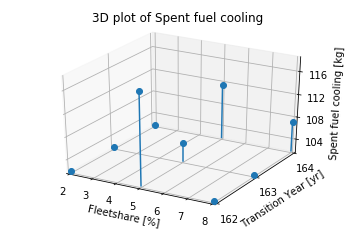
\includegraphics[width=0.58\linewidth]{figures/3d_sfc} 
        \caption{Inventory: Spent fuel cooling}
        \label{fig:3d_sfc}
    \end{subfigure}
    \begin{subfigure}[t]{0.58\textwidth}
        \centering
        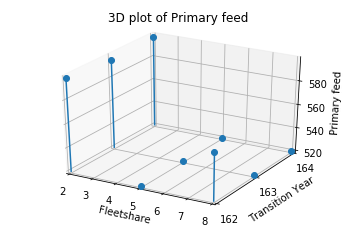
\includegraphics[width=\linewidth]{figures/3d_pf} 
        \caption{Inventory: Primary feed}
	    \label{fig:3d_pf}
    \end{subfigure}
    \begin{subfigure}[t]{0.58\textwidth}
        \centering
        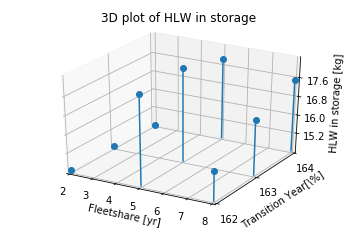
\includegraphics[width=\linewidth]{figures/3d_hlw} 
        \caption{Inventory: HLW in storage}
        \label{fig:3d_hlw}
    \end{subfigure}
    \caption{DYMOND EG01-30 Transition Scenario: ›Maximum amount of Pu [kg] in each inventory for varying fleet share and transition start date simulations \cite{chee_gwenchee/ddwrapper_2019}.}
\end{figure}

Figures \ref{fig:3d_sfc}, \ref{fig:3d_pf}, and \ref{fig:3d_hlw}
communicate how fleet share ratio and introduction date of advanced 
reactor technology 
synergistically impact maximum Pu in various inventories in the 
\gls{NFC}. 
Similar synergistic studies can be conducted for the output variables in 
all the evaluation metrics to better utilize this information for decision making. 
The results from each study can be normalized, weighted, and 
combined to create an optimization surface similar 
to Figure \ref{fig:passerini_payoff} to determine the ideal fleet share 
ratio and transition year combination. 

\subsubsection{\textbf{Cyclus}}
We evaluated 25 scenarios for a combination of PWR MOX fleet share percentage 
of 0\%, 5\%, 10\%, 15\%, 20\%, and advanced reactor introduction 
date of year 80 to 84.
Figures \ref{fig:cyclus_3d_hlw}, \ref{fig:cyclus_3d_depu}, and 
\ref{fig:cyclus_3d_ic}
visualize the final amount of HLW, the final amount of depleted uranium, 
and the total amount of idle capacity in the scenario for varying 
fleet share and advanced reactor introduction date values. 

Figure \ref{fig:cyclus_3d_hlw} shows that for scenarios in which 
there exists a smaller fleet share of \gls{MOX} \glspl{PWR}, and the 
transition begins later in the simulation, less high 
level waste produced. 
For a later transition year, we assume the initial 
\glspl{LWR} have a longer lifetime
and thus, advanced reactors exist in the simulation for a shorter 
amount of time, resulting in a smaller production of reprocessing 
HLW waste. 
Also, \gls{MOX} \glspl{PWR} produce more \gls{HLW} than \glspl{SFR}. 
Figure \ref{fig:cyclus_3d_depu} shows that as the introduction date 
of advanced reactors is pushed back, more depleted uranium is produced 
due to the extended lifetime of the \glspl{LWR} that utilize enriched 
natural uranium fuel that generates depleted uranium. 
Figure \ref{fig:cyclus_3d_ic} shows that idle capacity is minimized 
for a later advanced reactor introduction date. 
Having a later introduction date of advanced reactor technology ensures 
a sufficiently large inventory of transuranic elements is amassed
to produce fuel for the \gls{MOX} \glspl{PWR} and \glspl{SFR}.  
This ensures that there exists no gap in the supply chain resulting 
in idle advanced reactor capacity.

\begin{figure}[]
    \centering
    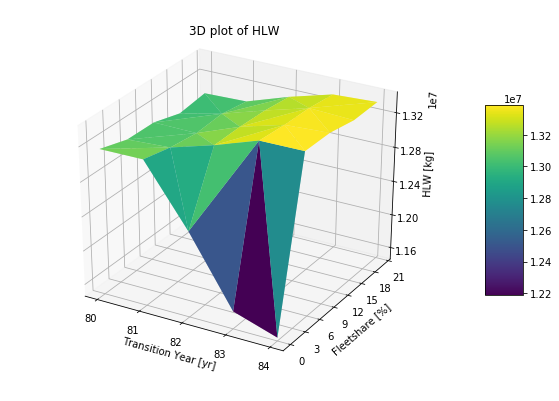
\includegraphics[width=0.8\linewidth]{cyclus_3d_hlw} 
    \caption{\Cyclus Transition Scenario: Final amount of HLW [kg] in the scenario for varying fleet share and transition start date simulations \cite{chee_arfc/dcwrapper_2019}.}
    \label{fig:cyclus_3d_hlw}
\end{figure}

\begin{figure}[]
    \centering
    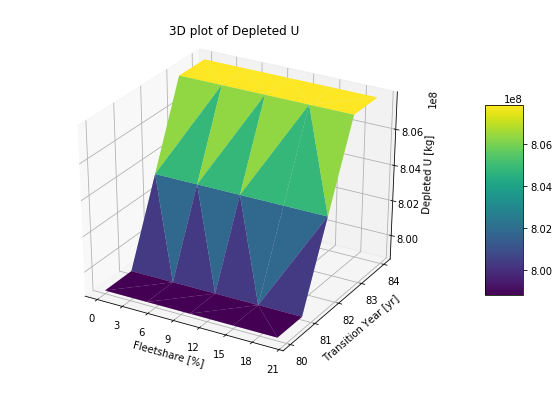
\includegraphics[width=0.8\linewidth]{cyclus_3d_depu} 
    \caption{\Cyclus Transition Scenario: Final amount of Depleted Uranium [kg] in the scenario for varying fleet share and transition start date simulations \cite{chee_arfc/dcwrapper_2019}.}
    \label{fig:cyclus_3d_depu}
\end{figure}

\begin{figure}[]
    \centering
    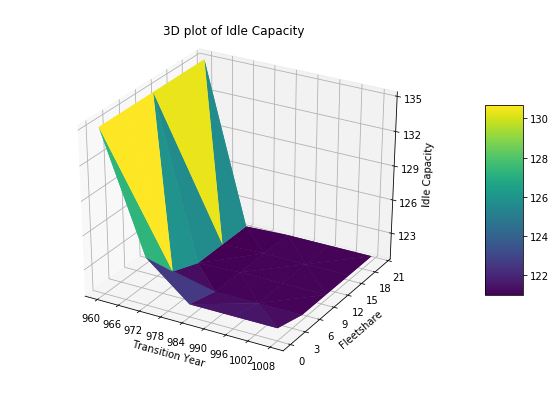
\includegraphics[width=0.8\linewidth]{cyclus_3d_ic} 
    \caption{\Cyclus Transition Scenario: Total amount of Idle Capacity [MW] in the scenario for varying fleet share and transition start date simulations \cite{chee_arfc/dcwrapper_2019}.}
    \label{fig:cyclus_3d_ic}
\end{figure}

\section{Global Sensitivity Analysis}
We used \texttt{dcwrapper} to conduct a global sensitivity 
analysis study to generate Sobol indices, which tells us which 
input parameters have the most influence on each output variable.
Section \ref{sec:sobol} describes this type of sensitivity 
analysis.
It provides a more holistic view of the system 
than OAT (section \ref{sec:oat}) and 
synergistic (section \ref{sec:synergistic}) sensitivity 
analysis because it decomposes the variance of the 
output of the scenario simulation into fractions which are 
attributed to each input, giving a better idea of the
most impactful input parameters. 
We could vary more than two variables in a synergistic 
sensitivity analysis, but it is difficult to visualize the results.

The input variables varied are fleet share ratio, 
transition start year, and used fuel cooling time.
The output variables considered are the final amount of HLW, 
the final amount of depleted uranium, and total idle capacity. 
Table \ref{tab:sobol} provides the Sobol indices which is 
a summary of the most influential input parameters 
for each output parameter. 
The Sobol indices are only comparable for each output variable 
(within each column). 
The fleet share has the largest impact on 
final HLW value, while the transition start year has the largest 
impact on final depleted uranium value and the total idle 
capacity value in the simulation. 
Transition start year and cooling time have some influence on 
the final value of HLW. 
Fleet share and cooling time do not influence the final 
depleted uranium value. 
    
    \begin{table}[]
        \centering
        \doublespacing
        \caption{Sobol Indices for a global sensitivity analysis study of the impact of 
        fleet share \% of PWR MOX reactors, transition start year and used fuel cooling time on various output
        variables: final amount of HLW, final amount of depleted uranium, and total 
        idle capacity in the simulation. The Sobol Indices are only comparable within each column, 
        not within each row \cite{chee_arfc/dcwrapper_2019}.}
        \label{tab:sobol}
            \small
            \begin{tabular}{l|lll}
                \hline	
                \multicolumn{4}{c}{\textbf{Sobol Indices for Output Variables}}   \\ \hline
                \textbf{Input Variables} & \textbf{Final HLW} & \textbf{Final Depleted Uranium} & \textbf{Total Idle Capacity} \\ \hline
                \textbf{Fleet Share} & 0.828     & 0                      & 0.00509             \\
                \textbf{Transition Year}                & 0.381     & 0.971                  & 1.505               \\
                \textbf{Cooling Time}                         & 0.126     & 0                      & 0                   \\ \hline

            \end{tabular}
    \end{table}

These global sensitivity analysis results give a good idea of the influence each 
input variable has on the output variables of interest. 
From Table \ref{tab:sobol}, we can inform the types of synergistic and one-at-a-time 
sensitivity analysis that should be done 
to understand the transition scenario system better. 
To better understand the impact of these three input parameters on final depleted 
uranium and total idle capacity, a one-at-a-time sensitivity analysis of transition 
year is sufficient. 
To better understand the impact of these three input parameters on the final HLW 
amount, a synergistic sensitivity analysis of share and cooling time is required.

\section{Main Takeaways}
\subsection{DYMOND Limitations}
For a transition scenario simulation in DYMOND, the user must 
manually edit the fuel management 
strategy to define which reactor the recycled 
part of each fuel type comes from for every year. 
Having the wrong fuel management strategy results in idle reactor
capacity due to the lack of fuel. 
Therefore, the user has to use trial and error to find a fuel 
management strategy to minimize or eliminate idle reactor capacity. 
With a 300-year simulation taking a few hours to run, it quickly 
becomes tedious and time-consuming.  

This issue impacts DYMOND sensitivity analysis 
because the fuel management strategy is 
optimized manually for specific scenario parameters, resulting in 
idle reactor capacity occurring when scenario parameters differs 
from it. 
An AI-based method (similar to \deploy) 
should be introduced to 
determine where the recycled part of each fuel comes from to 
minimize idle capacity in the simulation. 
This eases the setting up of transition scenarios, and enables 
more effective and accurate sensitivity analysis studies.

\subsection{Importance of Different Types of Sensitivity Analysis}
The OAT, synergistic, and global sensitivity analysis methods 
are all key to analyzing \gls{NFC} transition scenarios. 
In this chapter, we demonstrated each sensitivity analysis type. 
Each method has its advantage. 
When conducting a comprehensive sensitivity analysis of a specific 
transition scenario, 
global sensitivity analysis should be done first to 
determine which input variables are key to influencing the output 
variables of interest. 
OAT and synergistic sensitivity analysis can then be used together to 
do further analysis to determine the trends and quantitative impacts 
of specific input variables on specific output variables. 
Synergistic sensitivity analysis is useful for analyzing 
tightly coupled input variables.  
